\chapter{Цифровой двойник сетевых физических процессов}\label{ch:ch6}

\section{Цепь поставок}\label{sec:ch6/sect1}

\subsection{Big Data Analysis in Social Networks for Managing Risks}\label{subsec:ch6/sec1/sub1}

\paragraph{Introduction.} Nowadays clothing industry contributes noticeably to world-wide economy. Herewith large textile corporations sell primarily brands, not clothes itself. Thus, the main value for the modern clothing industry giants is a favourable consumer attitude \cite{Choi}. es itself. Hence, one of the main risks in the clothing industry is associated with the loss of confidence caused by negative feedback of customers \cite{IvanovDolguiSokolovIvanova,ChiuChoiDai}. Efficient risk management in such a field stems from analysis of consumer’s activities in social media \cite{Choi}. Indeed, deep analysis of activities in social media can enable decision-makers to obtain clear information on different risk aspects associated with a product that may cause a negative response from customers. Eventually, customer dissatisfaction may lead to a brand change. Mass brand reject may lead to financial loss and even bankruptcy of a textiles corporation \cite{TianChoiDing}.

Big data has been characterized in literature by 5Vs: volume, variety, velocity, veracity and value \cite{GunasekaranTiwariDubey}. Veracity and value are particularly important since data analysis shows the real value of big data. Big data analytics (BDA) is based on knowledge extraction from vast amounts of data, facilitating data-driven decision-making.

BDA has been undoubtedly the most elaborated area of digital technologies application to supply chain management over the last decade. Simchi-Levi and Wu \cite{SimchiLeviWu} analysed the application of BDA to retail and concluded that retailers must continuously strive to grow their revenue, margins and market share. Nguyen et al. \cite{NguyenZhouSpiegler} showed that optimization is the most popular approach in prescriptive analytics application to logistics and transportation area.

BDA applications to supply chain management can also be seen in procurement processes, manufacturing shop floors, promotion actions in the omnichannel model, routing optimization, real-time traffic operation monitoring and proactive safety management \cite{GunasekaranTiwariDubey,NguyenZhouSpiegler}. Papadopoulos et al. \cite{PapadopoulosGunasekaranDubey} pointed out that BDA can help in improving SC risk management and disasterresistance. Dolgui et al. \cite{DolguiIvanovSokolov} and Ivanov \cite{Ivanov} identified frameworks of risk management in the supply chains using digital technologies and data analytics.

Recent relevant implementation of big data analysis in social media (Twitter) to industry was made by Singh et al. \cite{SinghShuklaMishra}. They considered food industry and developed the approach which could inform supply chain decision-makers about customer feedback and issues in the flow/quality of food products.

Twitter information seems to be one of the most widely used data source for research and applications (see, for instance, \cite{ChenElmesChang} and \cite{BodrunovaLitvinenkoBlekanov}). In the context of brand management Twitter information was considered by Malhotra et al. \cite{MalhotraMalhotraSee}. Utilization of Twitter data is expanding in numerous directions from market prediction to public safety. Analysis of Twitter data has also been conducted by researchers in the domain of operation management \cite{TanZhanJi,FanNiu}.

This paper is devoted to investigation of Twitter information as an analytical basis for risk management in clothing industry. In particular, operational risks in the apparel supply chains are analysed which are usually concerned with demand and lead time fluctuations \cite{Ivanov,IvanovDolguiSokolov}.

\paragraph{Case study and Twitter data analysis.} The Twitter data analyzed in this research was used to understand issues related to risks identification in clothing supply chains. This analysis can help to illuminate reasons behind negative sentiments in discussions of Twitter users about sneakers. Sneakers are very popular footwear today which is discussed intensively. 

The total number of tweets extracted for this research was 248,728. They were captured from 01/09/2018 to 30/09/2018 using the keyword ‘sneakers’. Only tweets written in English language were considered, with no geographic constraint.

\begin{table} [htbp]%
	\centering
	\caption{Size of the discussion.}%
	\label{tab:discussionSize}% label всегда желательно идти после caption
	\renewcommand{\arraystretch}{1.6}%% Увеличение расстояния между рядами, для улучшения восприятия.
		\begin{tabulary}{\textwidth}{@{}>{\zz}L >{\zz}C@{}}% Вертикальные полосы не используются принципиально, как и лишние горизонтальные (допускается по ГОСТ 2.105 пункт 4.4.5) % @{} позволяет прижиматься к краям
			\toprule     %%% верхняя линейка
			Number of tweets & 248,728 \\ 
			Number of likes & 748,887  \\
			Number of retweets & 159,141 \\ 
			Number of comments & 125,747 \\ 
			\bottomrule %%% нижняя линейка
		\end{tabulary}%
\end{table}

The scale of the discussion depends not only on a total number of tweets but also on the value of discussion based on reaction of Twitter users to the topic. Indeed, total number of tweets without reaction of Twitter users can be associated with information attack or unfair market competition. Conversely, large amount of likes, retweets and comments means a discussion is of interest in Twitter community.

According to Table~\cref{tab:discussionSize}, discussion on sneakers is initiated by 248,728 tweets and, what is really important, generates 1,282,503 of total actions by Twitter users during one month. No doubt that it is indicative discussion and could be used for informative analyses. Figure~\cref{fig:activityTypes} visualizes that main contribution in the discussion activities is made by likes. This fact should be taken into consideration very carefully by analysts.

\begin{figure}[ht]
	\centerfloat{
		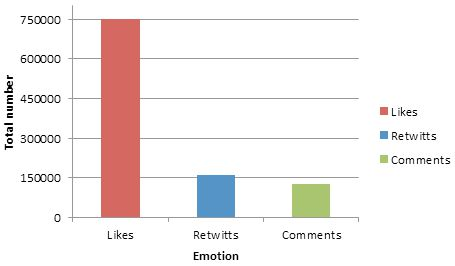
\includegraphics[scale=1.3]{activityTypes}
	}
	\caption{Types of activities.}\label{fig:activityTypes}
\end{figure}

Other important information to be extracted concerns number of real Twitter users involved in the discussion. This aspect is demonstrated in Table~\cref{tab:uniqueTwitterUsers}. Therefore, the discussion on sneakers in English-tweeting community during September of 2018 was initiated by 113,669 unique users, while 224,412 unique users take part in this discussion.

\begin{table} [htbp]%
	\centering
	\caption{Unique Twitter users.}%
	\label{tab:uniqueTwitterUsers}% label всегда желательно идти после caption
	\renewcommand{\arraystretch}{1.6}%% Увеличение расстояния между рядами, для улучшения восприятия.
	\begin{tabulary}{\textwidth}{@{}>{\zz}L >{\zz}C@{}}% Вертикальные полосы не используются принципиально, как и лишние горизонтальные (допускается по ГОСТ 2.105 пункт 4.4.5) % @{} позволяет прижиматься к краям
		\toprule     %%% верхняя линейка
		Number of unique tweeting users & 113,669 \\ 
		Number of unique users in the discussion & 224,412  \\
		\bottomrule %%% нижняя линейка
	\end{tabulary}%
\end{table}

Figure~\cref{fig:dailyTweetDynamics} demonstrates the dynamics of daily tweets devoted to sneakers during the September of 2018. The dynamics of the discussion has the peak in the beginning of month and then shows average fluctuation.

\begin{figure}[ht]
	\centerfloat{
		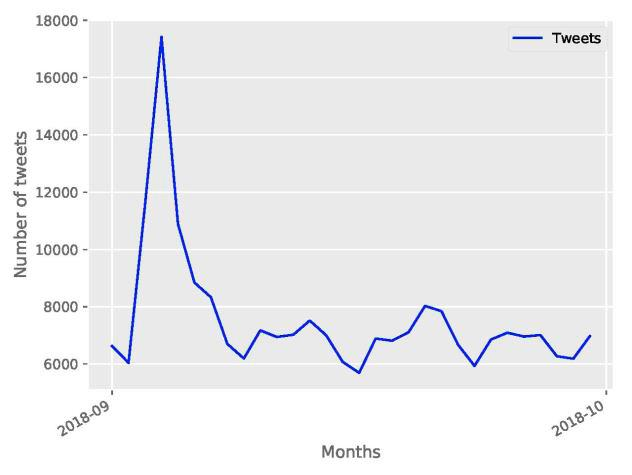
\includegraphics[scale=1]{dailyTweetDynamics}
	}
	\caption{Dynamics of daily tweets on sneakers in September 2018.}\label{fig:dailyTweetDynamics}
\end{figure}

Several hashtags were observed in the collected tweets. The most frequently used hashtags are highlighted in Table~\cref{tab:topHastags}.

\begin{table} [htbp]%
	\centering
	\caption{Top hashtags used.}%
	\label{tab:topHastags}% label всегда желательно идти после caption
	\renewcommand{\arraystretch}{1.6}%% Увеличение расстояния между рядами, для улучшения восприятия.
	\begin{adjustbox}{width=0.29\textwidth}
		\small
		\begin{tabulary}{\textwidth}{@{}>{\zz}L >{\zz}C >{\zz}C@{}}% Вертикальные полосы не используются принципиально, как и лишние горизонтальные (допускается по ГОСТ 2.105 пункт 4.4.5) % @{} позволяет прижиматься к краям
			\toprule     %%% верхняя линейка
			Hashtag & Freq (>100) & Freq(\%) \\
			\midrule %%% тонкий разделитель. Отделяет названия столбцов. Обязателен по ГОСТ 2.105 пункт 4.4.5
			\#sneakers & 1987 & 49.69 \\ 
			\#nike & 1077 & 26.93 \\
			\#sneakerhead & 680 & 17.00 \\ 
			\#kicks & 444 & 11.10 \\ 
			\#sneakerheads & 374 & 9.35 \\
			\#shoes & 343 & 8.58 \\
			\#sneaker & 331 & 8.28   \\ 
			\#kicksonfire & 322 & 8.05  \\
			\#jordan & 299 & 7.48 \\
			\#kotd & 269 & 6.73 \\ 
			\#airmax & 260 & 6.50 \\
			\#backtoschoolpic & 241 & 6.03 \\ 
			\#sneakeraddict & 241 & 6.03 \\
			\#athleisure & 227 & 5.68 \\
			\#ootd & 224 & 5.60 \\ 
			\#air & 211 & 5.28 \\
			\#sneakerfreak & 206 & 5.15 \\
			\#fashion & 195 & 4.88 \\
			\#airjordan & 195 & 4.88 \\
			\#sneakerfreaker & 184 & 4.60 \\
			\#shopmycloset & 161 & 4.03 \\
			\#soleretriever & 158 & 3.95 \\
			\#adidas & 157 & 3.93 \\
			\#mensfashion & 152 & 3.80 \\
			\#hypebeast & 148 & 3.70 \\
			\#sneakershopping & 138 & 3.45 \\
			\#sepatu & 124 & 3.10 \\
			\#lifestyle & 123 & 3.01 \\
			\#yeezy & 122 & 3.05 \\
			 \#fashionista & 121 & 3.03 \\
			\bottomrule %%% нижняя линейка
		\end{tabulary}%
	\end{adjustbox}
\end{table}

Keyword and hashtags allow for information accumulation on the topic. Hashtags demonstrate bright points of discussions. Herewith, a tweet consists of several words and carries semantic content. Big data analysis tool allows us to extract most frequently used words in tweets from considered set (table~\cref{tab:wordsUsed}).

\begin{table} [htbp]%
	\centering
	\caption{Words used in extracted tweets.}%
	\label{tab:wordsUsed}% label всегда желательно идти после caption
	\renewcommand{\arraystretch}{1.6}%% Увеличение расстояния между рядами, для улучшения восприятия.
	\begin{adjustbox}{width=0.25\textwidth}
		\small
		\begin{tabulary}{\textwidth}{@{}>{\zz}L >{\zz}C >{\zz}C@{}}% Вертикальные полосы не используются принципиально, как и лишние горизонтальные (допускается по ГОСТ 2.105 пункт 4.4.5) % @{} позволяет прижиматься к краям
			\toprule     %%% верхняя линейка
			Hashtag & Freq (>500) & Freq(\%) \\
			\midrule %%% тонкий разделитель. Отделяет названия столбцов. Обязателен по ГОСТ 2.105 пункт 4.4.5
			air & 9740 & 32.88 \\
			sneakers & 9657 & 32.60 \\
			nike & 6711 & 22.66 \\
			sneaker & 3385 & 11.43  \\
			max & 3147 & 10.62 \\
			jordan & 3128 & 10.56 \\
			mens & 2387 & 8.06 \\
			shoes & 2097 & 7.08 \\
			size & 1797 & 6.07 \\
			new & 1628 & 5.50 \\
			retro & 1382 & 4.67 \\
			white & 1209 & 4.08 \\
			black & 1118 & 3.77 \\
			force & 1048 & 3.54 \\
			running & 1005 & 3.40 \\
			ya & 971 & 3.28 \\   
			us & 873 & 2.95 \\
			di & 824 & 2.78 \\
			just & 792 & 2.67 \\
			via & 752 & 2.54 \\
			x & 729 & 2.46 \\
			now & 713 & 2.41 \\
			sneakerhead & 695 & 2.35 \\
			fashion & 687 & 2.32 \\
			ebay & 638 & 2.15 \\
			athletic & 628 & 2.12 \\
			amp & 607 & 2.05 \\
			check & 605 & 2.04 \\
			available & 594 & 2.01 \\
			brand & 593 & 2.00 \\			
			\bottomrule %%% нижняя линейка
		\end{tabulary}%
	\end{adjustbox}
\end{table}

Words extracted from tweets about sneakers occur in different combinations. Intellectual analysis, based on Biterm Topic Model, revealed seven macro topics which generate discussions \cite{BlekanovTarasovMaksimov}. Biterm Topic Model helps analysing a set of biterms (i.e., unordered word pair co-occurring in a short context). The main idea is that if two words co-occur more frequently, they are more likely to belong to a same topic \cite{YanyanJiafengXueqi}. Btm assumes the following generative process:
\begin{itemize}
	\item first, we draw distribution of tweets’ topics by distribution of Dirichlet,
	\item second, for each topic:
	\begin{itemize}
		\item we draw distribution of topics’ words by multino- mial distribution,
	\end{itemize}
	\item third, for each biterm:
	\begin{itemize}
		\item we draw distribution of biterms by multinomial
		distribution,
		\item we draw distribution of each term in this biterm separate multinomial distributions.
	\end{itemize}
\end{itemize}

As BTM does not model tweets explicitly, we need to provide a way to infer the topics in a tweet, i.e., evaluating the topic posterior. In this regard, we developed the chain rule based on Bayes’ formula and empirical distribution of words in a tweet.

As a result of the analysis seven topics were defined. Topic 1 unfolded around men sneakers. Twitter users share information about sizes and models, give positive and negative comments on the topic. Topics 2 and 3 can be characterized as meta-topics -- topics that do not contain any sense but express some artificially established patterns of the words. Topic 4 generates discussions around such model of sneakers as air. Topic 5 generates discussions around sales of amp and air sneakers. Topics 6 and 7 seem to be meta-topics too. Hot map of revealed topics is given in figure~\cref{fig:topicHotMap}.

\begin{figure}[ht]
	\centerfloat{
		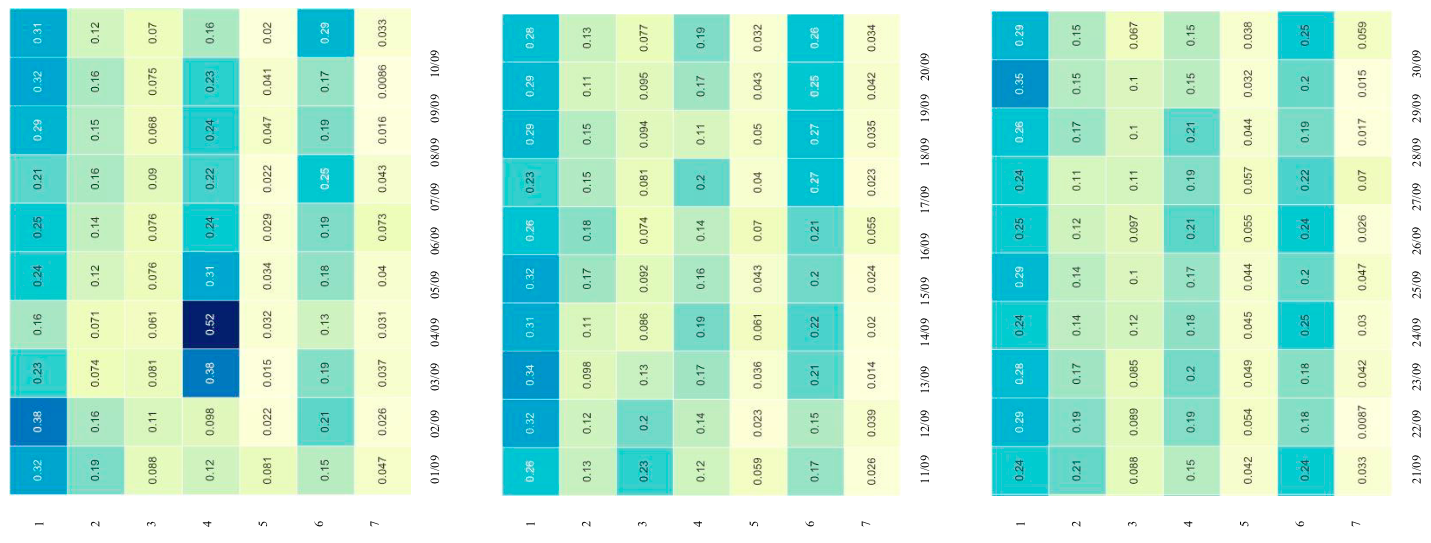
\includegraphics[angle=270, scale=0.5]{topicHotMap}
	}
	\caption{Hot map of topics devoted to sneakers in September 2018.}\label{fig:topicHotMap}
\end{figure}

From risk management perspectives negative tweets should be drifted apart from all others and analysed separately. During September of 2018 there were posted 14,181 negative tweets. Dynamic of negative tweets is given by figure~\cref{fig:dailyNegativeTweetDynamics}. Peak of negative feedback and hot discussion on topic 4 has direct correlation. Indeed, both peaks occur in the beginning of September. Therefore, it could be concluded that customers gave negative feedback in the beginning of September on topic 4. Semantic analysis defined that the main cause lies in disappointed expectation of customers. More precisely, new air sneakers were expected to be released but this did not happen (maybe customers just did not have accurate information on that). Anyway this caused irritation among customers that can be easily observed in many tweets. Thus, risk managers should take this situation into consideration and recommend to decision-makers to prevent leaks of information about new releases or make official statements in this regard in “on-line” regime.

\begin{figure}[ht]
	\centerfloat{
		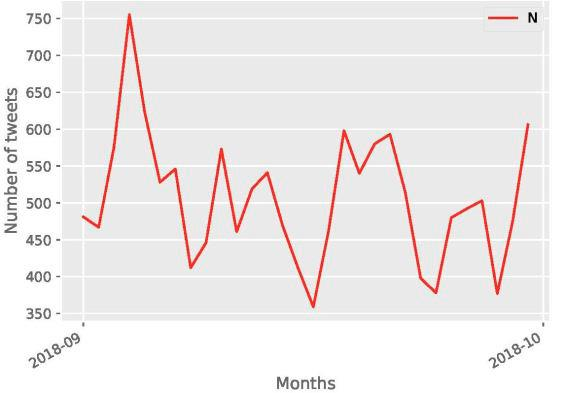
\includegraphics[scale=1.0]{dailyNegativeTweetDynamics}
	}
	\caption{Dynamic of daily negative tweets devoted to sneakers in September 2018.}\label{fig:dailyNegativeTweetDynamics}
\end{figure}

\paragraph{Managerial implications.} Social networks became insistently important source for different types of information. Nevertheless, the considered case study showed how much extended data analysis is required to establish informative issues for revealing risk points from Twitter. The investigated case study pertains to the following conclusion: textiles corporations should increase their presence in social networks to minimize operational risks. Therefore, in spite of its complexity big data analysis of social networks could be valuable source of information for risk managers and decision-makers at different levels in textiles industry.

\paragraph{Conclusion.} Social networks are increasingly affecting various aspects of human life. Thus social networks also impact different economic processes. In this paper, the case study in the segment of footwear supply chain was analysed, where data from Twitter was used for a period of one month. Analysis showed that discussion contains more than one million activities in Twitter devoted to the considered keyword. Such amount of activities should not be ignored while minimizing risks in clothing distribution by textiles corporations. In future work we are planning to extend our research and investigate social network data analysis for longer period of times and a broad product range to contribute to decision-making support in supply chain risk management.

\section{Визуализация}\label{sec:ch6/sect2}

\section{Геопозиция}\label{sec:ch6/sect3}

\section{Сеть маршрутов распространения физических ресурсов на основе данных (обработанных подсетью виртуальных сетевых агентов)}\label{sec:ch6/sect4}

\FloatBarrier

